%! TEX root = **/010-main.tex
% vim: spell spelllang=en:

\section{Results}

\subsection{Replicating results from Kutznetsov et al.}

To analyze the performance of the program the system found by Kutznetsov et al.
\cite{kuznetsov_visualization_2013} will be used.
\footnote{This system is the same that was previously discussed
in~\cref{sec:context} (\cref{fig:kuznetsov})}

\Cref{eq:kuznetsov} shows the system and its parameters and \cref{fig:kuznetsov2}
shows the limit cycles.

\begin{equation}%
    \label{eq:kuznetsov}
    \begin{split}
        \frac{dx}{dt} &= x^2 + xy + y^2 + x + y\\
        \frac{dy}{dt} &= ax^2 + bxy * cy^2 + \alpha x \beta y
    \end{split}
    \qquad \qquad
    \begin{split}
        a &= -10\\
        b &= 2.2\\
        c &= 0.7\\
        \alpha &= -72.7778\\
        \beta &= 0.0015
    \end{split}
\end{equation}

\begin{figure}[H]
    \centering
    \includegraphics[width=1.0\textwidth]{4cycles}
    \caption{Visualization of four limit cycles in two-dimensional polynomial quadratic system, from Ref.~\cite{kuznetsov_visualization_2013}
    }%
    \label{fig:kuznetsov2}
\end{figure}

\pagebreak
\Cref{fig:kuznetsov_cuda} shows a visualization of the points which a ratio
equal to one with tolerance $10^{-6}$. These correspond exactly with the results
of~\cite{kuznetsov_visualization_2013}. The computation of this data took 250ms
and using a grid of $1024 \times 1024$ trajectories, and a fixed \emph{Runge Kutta}
of third order with a step size of $10^{-3}$. Notice that some points left of $x
= 0$ are not found. Nevertheless, the cycles can be identified easily. Notice that the
4th limit cycle which should be to the left of our plot cannot be found by the program
due to the stiffness of the system on that area. This problem is discussed in more detail
in~\cref{sub:stiffness}. For the rest of the analysis we will only consider
these 3 limit cycles.

\begin{figure}[H]
    \centering
    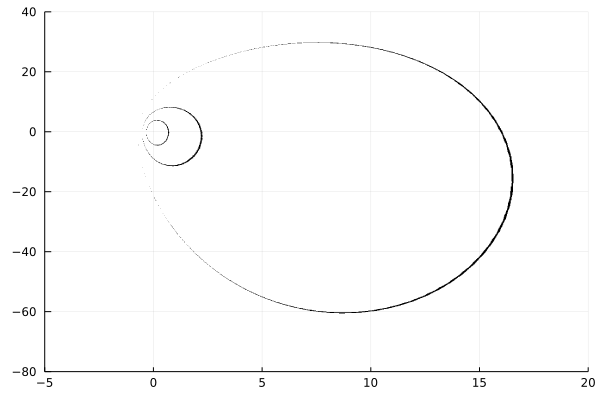
\includegraphics[width=0.8\textwidth]{kutznetsov_cuda}
    \caption{Limit cycles found using our program ($1024^2$ grid)}%
    \label{fig:kuznetsov_cuda}
\end{figure}

Using a bigger grid size of $5000\times5000$, we obtain clearer results but it takes
1200ms. There is not much benefit in this instance since the cycles are clear and
we are searching inside a well delimited plane, but when the search space is greater
it does offer a benefit.

\begin{figure}[H]
    \centering
    \includegraphics[width=0.8\textwidth]{kutznetsov_cuda_5k}
    \caption{Limit cycles found using our program ($5000^2$ grid)\\
        Black areas correspond to points from which trajectories have
        a rate of 1 (tol $10^{-6}$)
    }%
    \label{fig:kuznetsov_cuda_5k}
\end{figure}

\paragraph{Clustering}

\Cref{fig:histograms} shows the distribution of the 4 different local extrema
values associated with all points with rate of change equal to 1 (with tolerance
$1^{-6}$), we can see that there are 3 clear groups in each one of the local extrema.

If we compute the \emph{K-means} for 3 clusters we obtain the cluster centers shown
in~\cref{tab:clusters}. \Cref{fig:bounding} shows the bounding boxes defined by the
clusters obtained as an overlay over \cref{fig:kuznetsov_cuda}.


\begin{figure}[H]
    \centering
    \includegraphics[width=0.8\textwidth]{histograms}
    \caption[Distribution values for local extrema]%
    {Histogram of distribution of values for each local extrema with rate of
        change equal to 1 (tol $1^{-6}$).
    }%
    \label{fig:histograms}
\end{figure}

\begin{table}[H]
    \centering
    \caption{Cluster centers}%
    \label{tab:clusters}
    \begin{tabular}{crrrr}
        \toprule
        Cluster & $x_{\min}$ & $x_{\max}$ & $y_{\min}$ & $y_{\max}$ \\ \midrule
        A & -0.716937 & 16.4835  & -60.2806  & 29.7273 \\
        B & -0.521985 &  2.20031 & -11.3237  &  8.17958 \\
        C & -0.338311 &  0.68522 &  -4.48625 &  3.84119 \\
        \bottomrule
    \end{tabular}
\end{table}

\begin{figure}[H]
    \centering
    \includegraphics[width=0.8\textwidth]{bounding}
    \caption{Bounding boxes defined by the clusters in \cref{tab:clusters}
        overlaid on top of \cref{fig:kuznetsov_cuda}
    }%
    \label{fig:bounding}
\end{figure}

\pagebreak
\subsection{Applying slight modifications}

\Cref{fig:bounding_a10_1} shows the result of finding limit cycles in the same
system used in the previous examples (\cref{eq:kuznetsov}) but with a slight modification
of parameter $a$ from 10 to 10.1. We can see that the cycles are slightly more similar in size.
Changing to 10.2 only one cycle remains. With $a = 9.9$ there are only two cycles. Other slight
modifications of the other parameters also reduce the number of cycles.

\begin{figure}[H]
    \centering
    \includegraphics[width=0.8\textwidth]{bounding_a10_1}
    \caption{Limit cycles found on system \cref{eq:kuznetsov} with parameter
        $a$ modified from $10.0 \to 10.1$
    }%
    \label{fig:bounding_a10_1}
\end{figure}

\pagebreak
\subsection{Changing window range}
The previous figures all searched for limit cycles inside the range:
$x \in (-5, 20), y \in (-60, 40)$. In the following section an analysis on the
capacity of the program to find the cycles with different windows will be performed.

\paragraph{Bigger area}

\begin{figure}[H]
    \centering
    \includegraphics[width=0.8\textwidth]{bounding_100x100}
    \caption{Limit cycles found on system from \cref{eq:kuznetsov} \\
        ($1024 \times 1024$ grid over $x, y \in (-100, 100)$)
    }%
    \label{fig:bounding_100x100}
\end{figure}

As shown in~\cref{fig:bounding_100x100}, with a window of $x,y \in (-100,100)$
we obtain the clusters without problem. Increasing the window further to
$(-1000, 1000)$ does only find the two bigger limit cycles. A possible optimization
could be to make two pases, one to find the bigger limit cycles and a second one using
as a window the bounding box of the limits found.

\pagebreak
\paragraph{Partial occlusion}

The algorithm should be robust to partial occlusion of the cycle, meaning that
even if part of the cycle is outside the window it should still be detected.
In~\cref{fig:bounding_occ} we show an image of the results applied with a window
of $x \in (0, 5), y \in (0, 20)$ (Shown in gray). The clusters are equivalent as
the ones in the previous examples. Note that the line of the biggest cluster is very thin
since there are not many points. As long as the window contains enough part of the trajectory of
a limit cycle\footnote{And the trajectory is not stiff (see \cref{sub:stiffness})} with
enough resolution, the cycles can be identified.

\begin{figure}[H]
    \centering
    \includegraphics[width=0.8\textwidth]{bounding_occlusion}
    \caption{Limit cycles found on system from \cref{eq:kuznetsov} \\
        ($1024 \times 1024$ grid over $x \in (0, 5), y \in (0, 20)$)
    }%
    \label{fig:bounding_occ}
\end{figure}

\pagebreak
\paragraph{Compactified plane}

Since the plane in $\mathcal{R}^2$ is infinite, in order to visualize limit cycles without
restricting portions of the plan a compactification should be performed.
In \cref{sec:compact-stiff} there is a more in depth explanation of how this can be done. In
our case the compactificaction is rather simple and just involves calculating the tangent,
reducing the plane from $(-\infty, \infty)$  to $(-\pi/2, \pi/2)$. This compactification is
not ideal since it deforms the plane a lot, but allows to perform a more wide search of cycles.
Although it does not help if they are big since they get \emph{squished} on the borders. The
result of applying the tangent compactification and running the program is shown
in~\cref{fig:bounding_compact}. The biggest cycle is almost non visible despite the fact that
it is not particularly big ($y_{\min} \approx -60, y_{\max} \approx 30$).

\begin{figure}[H]
    \centering
    \includegraphics[width=0.8\textwidth]{bounding_compact}
    \caption{Limit cycles found on system from \cref{eq:kuznetsov} \\
        ($1024 \times 1024$ grid over compactified plane)
    }%
    \label{fig:bounding_compact}
\end{figure}
